% !TeX document-id = {1d88a3b2-9b5b-461b-9b0a-590d1c20474b}
% !TeX TXS-program:compile = txs:///pdflatex/[--shell-escape]
\documentclass[border={0 0mm 0 -1mm}]{standalone}
\usepackage{amsmath,amsfonts,amssymb}
\usepackage{tikz,pgfplots}
\usetikzlibrary{arrows,arrows.meta,bending,calc,decorations,shadings,shadows,shapes,shapes.arrows,shapes.geometric}
\usetikzlibrary{calc,fadings,decorations.pathreplacing}
\usepgfplotslibrary{units,fillbetween,groupplots,colorbrewer}
\usetikzlibrary{pgfplots.colorbrewer,}
\usetikzlibrary{arrows,decorations.pathmorphing,perspective}
\usepackage{pgfplotstable}
\usetikzlibrary{3d,spy}

\newcommand*{\xMin}{0}%
\newcommand*{\xMax}{10}%
\newcommand*{\yMin}{0}%
\newcommand*{\yMax}{7}%

\definecolor{As}{RGB}{255,255,0}
\definecolor{Al}{RGB}{173,216,230}
\definecolor{Ga}{RGB}{0,128,150}
\begin{document}
	
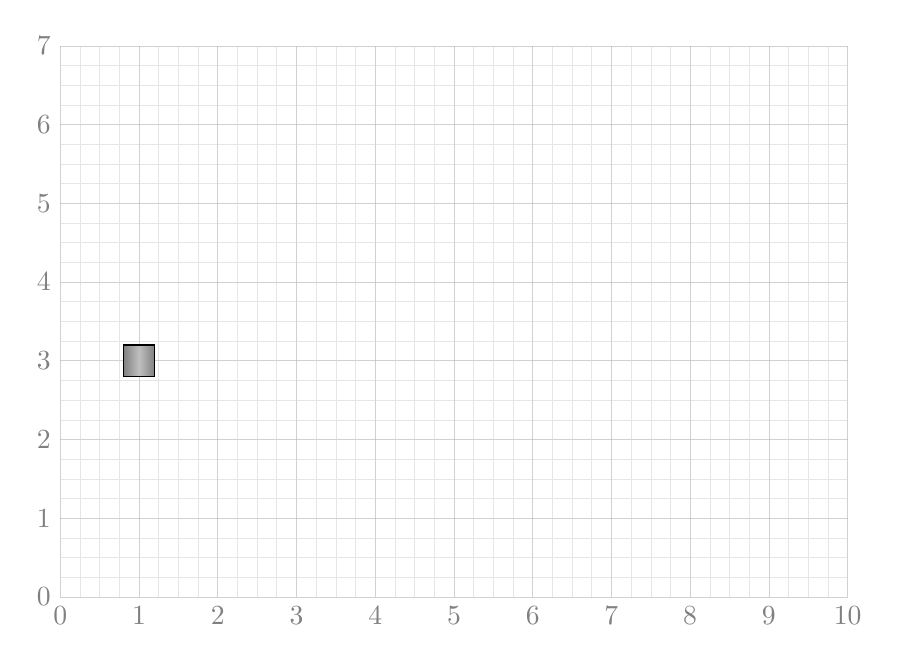
\begin{tikzpicture}
								\draw[step=.25cm,gray,very thin,opacity=0.2] (0,0) grid (\xMax,\yMax);
										 \foreach \i in {\xMin,...,\xMax} {
														\draw [very thin,gray,opacity=0.2] (\i,\yMin) -- (\i,\yMax)  node [below,opacity=1] at (\i,\yMin) {$\i$};
													}
										\foreach \i in {\yMin,...,\yMax} {
														\draw [very thin,gray,opacity=0.2] (\xMin,\i) -- (\xMax,\i) node [left,opacity=1] at (\xMin,\i) {$\i$};
													}
				



	
%\begin{scope}[perspective,rotate around y=-15]
%\draw[fill=yellow ] (0,2)--(2,2)--(2,4)--(0,4)--cycle;
%\draw[fill=yellow ] (0,4)--(1,5)--(3,5)--(2,4)--cycle;
%\draw[fill=yellow ] (3,5)--(3,3)--(2,2)--(2,4)--cycle;
%\end{scope}


%\begin{scope}[xshift=0cm,yshift=0cm]
%%
%\draw[left color = black!50, right color = black!50,middle color = black!25] (0,2.9)--(2,2.9)--(2,3.1)--(0,3.1)--cycle;
%\draw[left color = black!50, right color = black!50,middle color = black!25] (2,2.9)--(3,3.9)--(3,4.1)--(2,3.1)--cycle;
%\draw[left color = black!50, right color = black!50,middle color = black!25] (0,3.1)--(2,3.1)--(3,4.1)--(1,4.1)--cycle;
%\draw[opacity=0.5,draw=gray,fill=yellow,fill opacity=0.5 ] (0,2)--(2,2)--(2,4)--(0,4)--cycle;
%\draw[opacity=0.5,draw=gray,fill=yellow,fill opacity=0.5 ] (0,4)--(1,5)--(3,5)--(2,4)--cycle;
%\draw[opacity=0.5,draw=gray,fill=yellow,fill opacity=0.5 ] (3,5)--(3,3)--(2,2)--(2,4)--cycle;	
%
%\end{scope}

%\begin{scope}[xshift=0cm,yshift=0cm]
%	%
%	\draw[left color = black!50, right color = black!50,middle color = black!25] (0,2.9)--(2,2.9)--(2,3.1)--(0,3.1)--cycle;
%	\draw[left color = black!50, right color = black!50,middle color = black!25] (2,2.9)--(3,3.9)--(3,4.1)--(2,3.1)--cycle;
%	\draw[left color = black!50, right color = black!50,middle color = black!25] (0,3.1)--(2,3.1)--(3,4.1)--(1,4.1)--cycle;
%	\draw[opacity=0.5,draw=gray,fill=yellow,fill opacity=0.5 ] (0,2)--(2,2)--(2,4)--(0,4)--cycle;
%	\draw[opacity=0.5,draw=gray,fill=yellow,fill opacity=0.5 ] (0,4)--(1,5)--(3,5)--(2,4)--cycle;
%	\draw[opacity=0.5,draw=gray,fill=yellow,fill opacity=0.5 ] (3,5)--(3,3)--(2,2)--(2,4)--cycle;	
%	
%	
%\end{scope}

\begin{scope}[xshift=0cm,yshift=0cm]
	%
	\draw[left color = black!50, right color = black!50,middle color = black!25] (0.8,2.8)--(1.2,2.8)--(1.2,3.2)--(0.8,3.2)--cycle;
%	\draw[left color = black!50, right color = black!50,middle color = black!25] (
%	1.2,2.8)--(3,3.8)--(3,4.2)--(1.2,3.2)--cycle;
%	\draw[left color = black!50, right color = black!50,middle color = black!25] (0.8,3.2)--(1.2,3.2)--(3,4.2)--(2.5,4.2)--cycle;
	%\draw[opacity=0.5,draw=gray,fill=yellow,fill opacity=0.5 ] (0,2)--(2,2)--(2,4)--(0,4)--cycle;
	%\draw[opacity=0.5,draw=gray,fill=yellow,fill opacity=0.5 ] (0,4)--(1,5)--(3,5)--(2,4)--cycle;
	%\draw[opacity=0.5,draw=gray,fill=yellow,fill opacity=0.5 ] (3,5)--(3,3)--(2,2)--(2,4)--cycle;	
	
	
\end{scope}

\end{tikzpicture}
	
	
\end{document}